\chapter{Modelare și proiectare}

\section{Cazurile utilizatorului și diagrame}
\label{sec:ch3sec1}
 \par Există un sigur tip de utilizator care poate avea interacțiune cu aplicația, pe viitor se poate dezvolta încă un tip de utiizatoracesta având scopul de a administra aplicația. Fiecare utilizator are un nume unic și o parolă pentru a se conecta la aplicație, acolo unde el poate să: caute filme, să își creeze propia lui lista cu filme, să dea notă la un film sau să vadă detalii despre un film acolo unde sunt prezente și recomandări pentru filmul respectiv.
		\begin{figure}[htbp]
			\centerline{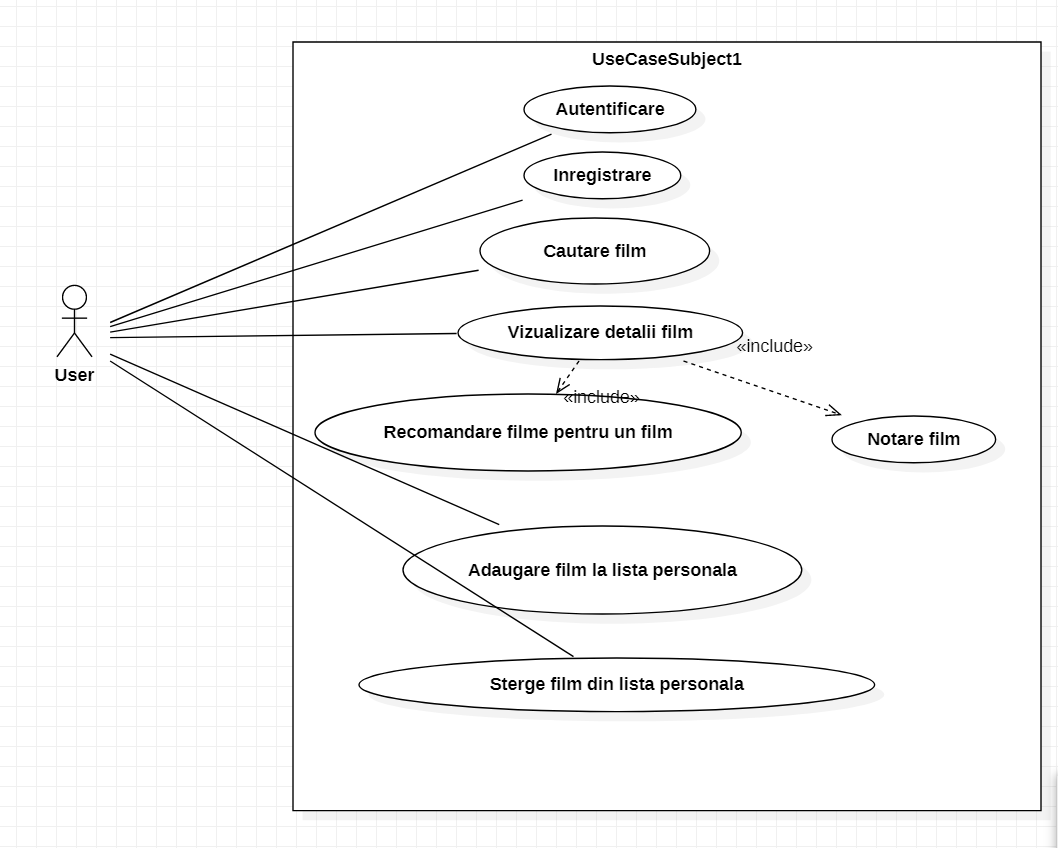
\includegraphics[width=13cm, height=10cm]{figures/use case.png}}
			\caption{Diagrama de cazuri}
			\label{fig}
		\end{figure}
\newline
\newline
\par \textbf{Figura 1}: Diagrama secvențială înregistrare
		\begin{figure}[htbp]
			\centerline{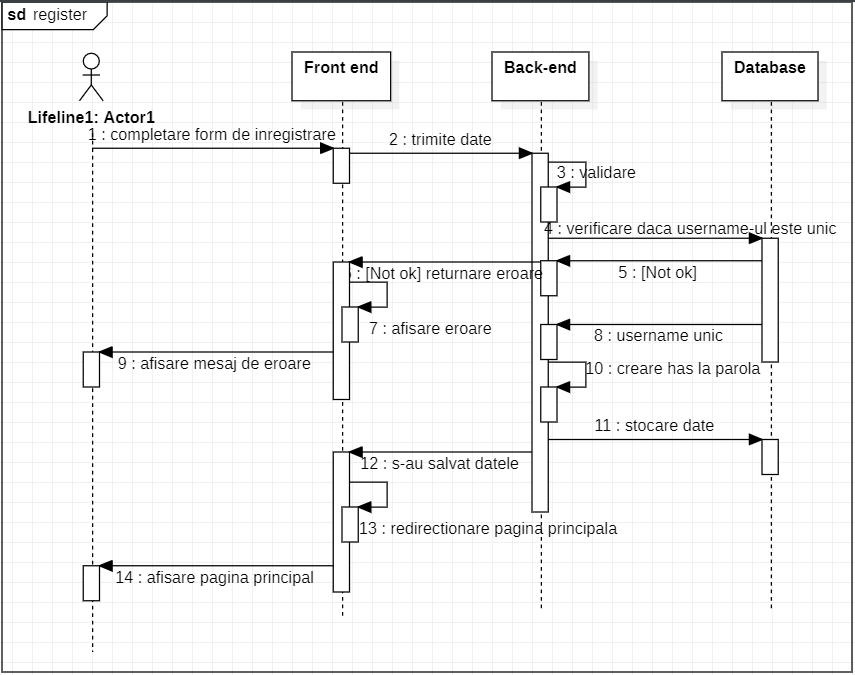
\includegraphics[width=13cm, height=8cm]{figures/sec register.png}}
			\caption{Diagrama secvențială pentru înregistrare}
			\label{fig}
		\end{figure}

\par \textbf{Figura 2}: Diagrama secvențială autentificare
		\begin{figure}[htbp]
			\centerline{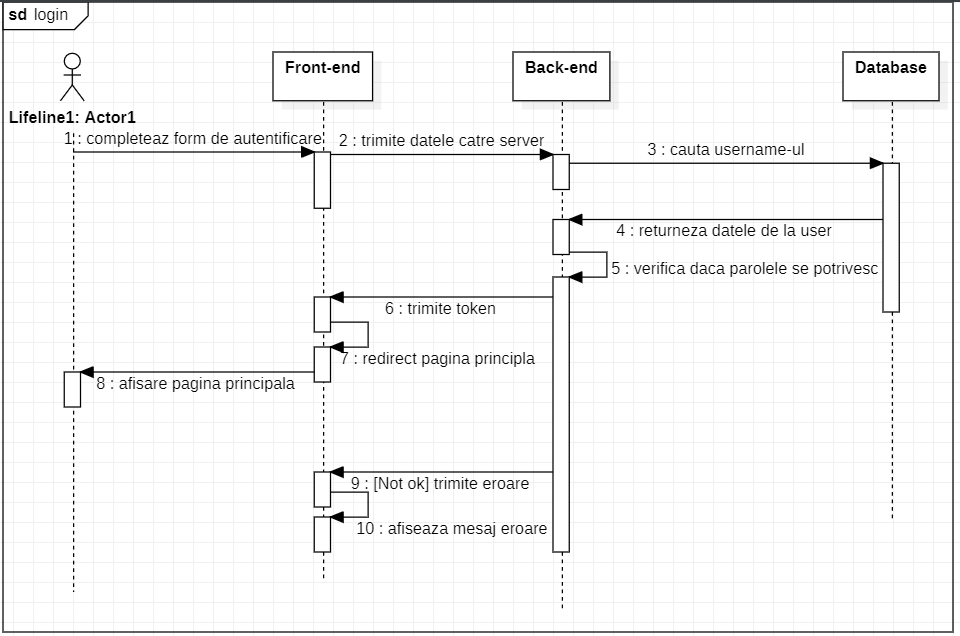
\includegraphics[width=13cm, height=8cm]{figures/login diagrma secventiala.png}}
			\caption{Diagrama secvențială pentru autentificare}
			\label{fig}
		\end{figure}
\newline
\newline
\newline
\newline
\newline
\par \textbf{Figura 3}: Diagrama secvențială adaugare film la lista personală
		\begin{figure}[!h]
			\centerline{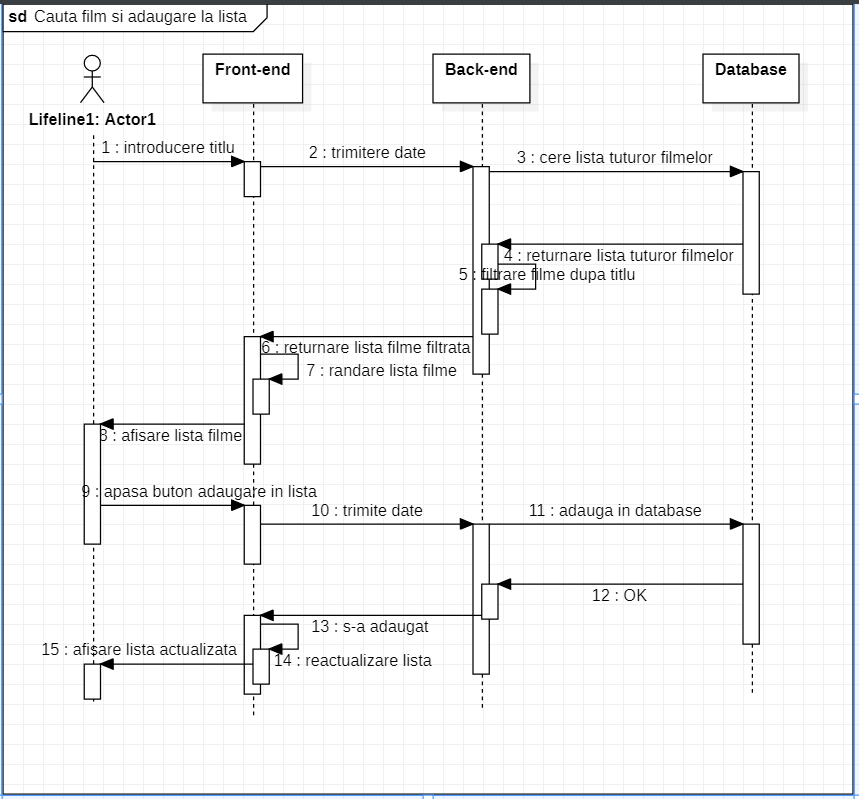
\includegraphics[width=14cm, height=10cm]{figures/cauta si adauga.png}}
			\caption{Diagrama secvențiala adaugare film la lista}
			\label{fig}
		\end{figure}

\par \textbf{Figura 4}: Diagrama secvențială adaugare film la lista personală
		\begin{figure}[!h]
			\centerline{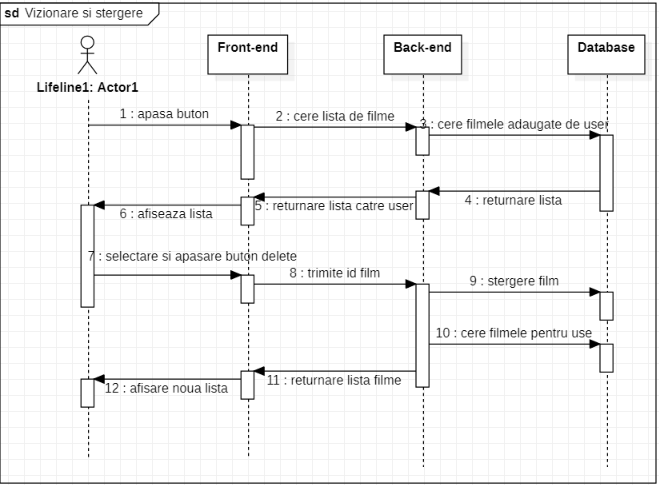
\includegraphics[width=14cm, height=10cm]{figures/fig.png}}
			\caption{Diagrama secvențială adaugare film la listă}
			\label{fig}
		\end{figure}

\par \textbf{Figura 5}: Acordare rating
		\begin{figure}[!h]
			\centerline{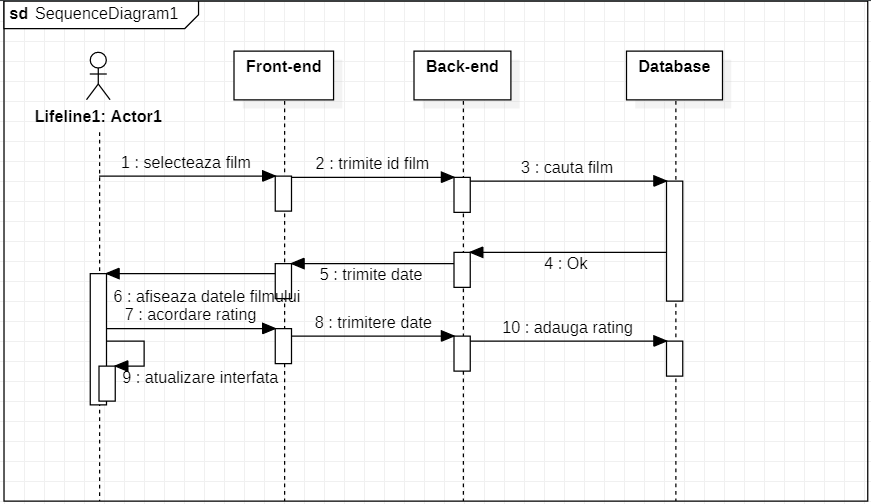
\includegraphics[width=14cm, height=10cm]{figures/acordare rating.png}}
			\caption{Diagrama secvențială adaugare film la listă}
			\label{fig}
		\end{figure}

\par \textbf{Figura 6}: Recomandare filme pentru un film
		\begin{figure}[!h]
			\centerline{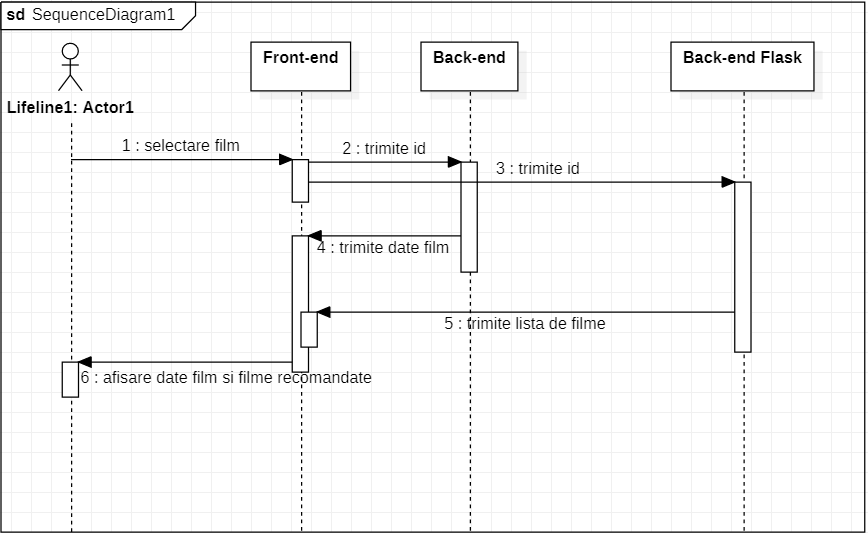
\includegraphics[width=14cm, height=10cm]{figures/recomandarea de filme.png}}
			\caption{Diagrama secvențială adaugare film la listă}
			\label{fig}
		\end{figure}

\par \textbf{Figura 6}: Recomandare filme pentru un o lista de filme
		\begin{figure}[!h]
			\centerline{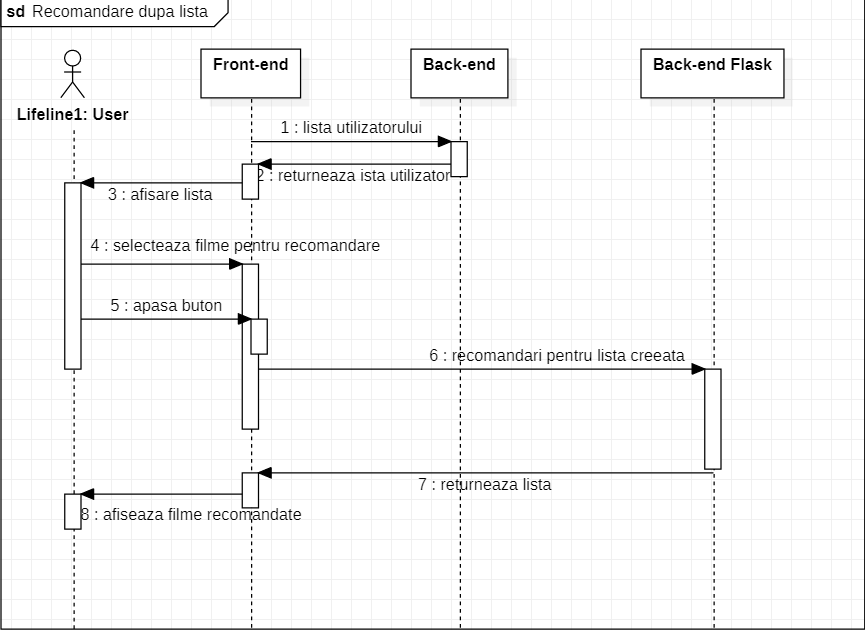
\includegraphics[width=14cm, height=10cm]{figures/rec.png}}
			\caption{Diagrama secvențială recomandare filme pentru o lista de filme}
			\label{fig}
		\end{figure}

\section{Utilizarea aplicației}
\label{sec:ch3sec2}
\par Când utilizatorul aceseaza siteul acesta este redirecționat către pagină de autentificare, dacă acesta nu are cont poate apăsa pe butonul Register și va fi redirecționat către o pagină care conține un formular de înregistrare. După ce toate datele au fost completate și înregistrarea a fost făcută cu succes acesta va fi redirecționat înpoi către pagină de autentificare, unde se poate autentifica cu noile credențiale.
\par După autentificare, utilizatorul este redirecționat către pagina principală unde în dreapta are un meniu de navigare și în centrul paginii o bară de căutare. Pe pagina principală utilizatorul poate să își caute filme, după introducerea unui titlu și apăsarea butonului de căutare i se vor afișa o listă cu toate filmele ce conțin în titlu șirul de caractere introduse de utilizator. Pe această pagină un film poate avea una sau două posibilități: să se vadă detalii despre film sau să fie adăugat la lista personală de filme.
\par Dacă se apasă pe butonul de Detalii la un film utilizatorul este redirecționat către pagina unde se pot vedea detaliile unui film, cum ar fi: titlu, descriere, actorii care joacă în film, țara de origine a filmului, directorii filmului, genurile, scriitorii care au venit cu idei pentru film, rating-ul general al filmului care reprezintă media notelor date de ceilanți utilizatori și cel mai important lucru se poate vedea patru filme recomandate pentru filmul respectiv. Tot pe această pagină se poate acordă o notă filmului influențând de altfel și nota generală a filmului.
\par Dacă se apasă pe butonul de adăugare la lista personală filmul va fi adăugat, iar butonul respectiv va dispărea. Pentru a vedea această lista din meniul din dreapta se poate naviga către pagina în care se prezintă lista cu filme adăugate de utilizator. Aceste filme tot două butoane: unul de ștergere care șterge filmul din lista și același buton de detalii că pe pagina principală. Tot pe această pagină utilizatorul își poate creea o sub lista din lista personală, iar la apăsarea butonului de recomandare acesta va primi o serie de filme recomandate pentru ce a ales în sublista lui.

